\documentclass[12pt,a4paper,oneside]{report}

\usepackage[a4paper,top=1in,bottom=1in,left=1.25in,right=1in]{geometry}
\usepackage[T1]{fontenc}
\usepackage[utf8]{inputenc}
\usepackage{newtxtext,newtxmath}
\usepackage{setspace}
\usepackage{indentfirst}
\usepackage{titlesec}
\usepackage{graphicx}
\usepackage{float}
\usepackage{booktabs}
\usepackage{longtable}
\usepackage{array}
\usepackage{multirow}
\usepackage{enumitem}
\usepackage{amsmath}
\usepackage{tikz}
\usetikzlibrary{arrows.meta,positioning,shapes.geometric,fit,calc}
\usepackage{hyperref}
\usepackage{fancyhdr}
\usepackage{caption}
\usepackage{listings}
\usepackage{xcolor}
\graphicspath{{../ref images/}{ref images/}}

\setlength{\parindent}{0.2in}
\setlength{\parskip}{0pt}
\onehalfspacing
\captionsetup{font=normalsize,labelfont=bf}
\setcounter{secnumdepth}{3}
\setcounter{tocdepth}{3}

\titleformat{\chapter}[display]
{\centering\bfseries\fontsize{16pt}{18pt}\selectfont}
{\chaptertitlename\ \thechapter}{8pt}{\MakeUppercase}

\titleformat{\section}
{\bfseries\fontsize{14pt}{16pt}\selectfont\MakeUppercase}
{\thesection}{0.8em}{}

\titleformat{\subsection}
{\normalfont\fontsize{12pt}{14pt}\selectfont}
{\thesubsection}{0.8em}{}

\pagestyle{fancy}
\fancyhf{}
\fancyfoot[C]{\thepage}
\renewcommand{\headrulewidth}{0pt}

\hypersetup{
  colorlinks=true,
  linkcolor=black,
  citecolor=black,
  urlcolor=blue
}

\lstdefinestyle{reportcode}{
  basicstyle=\ttfamily\small,
  breaklines=true,
  frame=single,
  numbers=left,
  numberstyle=\tiny,
  keywordstyle=\color{blue!70!black},
  commentstyle=\color{green!40!black},
  stringstyle=\color{red!60!black},
  tabsize=2
}

\begin{document}

\begin{titlepage}
\centering
{\Large PROJECT REPORT\par}
\vspace{1cm}
{\bfseries\LARGE JOBEASE\par}
\vspace{0.5cm}
{\large AUTOMATED JOB APPLICATION ASSISTANT FOR NAUKRI CAMPUS\par}
\vspace{1.2cm}
{\large Submitted in partial fulfilment of the requirement for the award of the degree of\par}
\vspace{0.5cm}
{\bfseries\Large BACHELOR OF TECHNOLOGY\par}
\vspace{0.3cm}
{\large IN\par}
\vspace{0.3cm}
{\large COMPUTER SCIENCE \& ENGINEERING\par}
\vspace{1.0cm}
{\large Submitted by\par}
\vspace{0.4cm}
{\large NAME 1 -- University Roll No. XXXXXXXX\par}
{\large NAME 2 -- University Roll No. XXXXXXXX\par}
\vspace{1.0cm}
{\large Under the guidance of\par}
\vspace{0.4cm}
{\large Mr. XYZ\par}
{\large Designation\par}
\vfill
{\large Project Group No: XX\par}
{\large Department of Computer Science and Engineering\par}
{\large Graphic Era Hill University\par}
{\large May, 2026\par}
\end{titlepage}

\chapter*{Candidate's Declaration}
\addcontentsline{toc}{chapter}{Candidate's Declaration}
I/We hereby certify that the work presented in this project report entitled \textbf{``JobEase: Automated Job Application Assistant for Naukri Campus''}, submitted in partial fulfilment of the requirements for the award of the Degree of Bachelor of Technology in Computer Science and Engineering, is an authentic record of the work carried out by us under the supervision of the project guide in the Department of Computer Science and Engineering, Graphic Era Hill University, Dehradun. The ideas, implementation details, experimental observations, and results presented in this report are original to the best of our knowledge and have not been submitted in full or part for the award of any other degree or diploma.

The report has been prepared after conducting careful requirement study, designing a modular and scalable software architecture, implementing the mobile application and automation backend, and validating the system through realistic execution scenarios on the Naukri Campus portal. We further declare that all external references, published sources, and technical materials used for conceptual understanding have been duly acknowledged in the references section.

\vspace{1.2cm}
\noindent Name 1 \hfill University Roll No. XXXXXXXX \hfill Signature\\[1.0cm]
\noindent Name 2 \hfill University Roll No. XXXXXXXX \hfill Signature

\chapter*{Acknowledgement}
\addcontentsline{toc}{chapter}{Acknowledgement}
We express our sincere gratitude to our project guide, \textbf{Mr. XYZ}, for his continuous mentoring, constructive reviews, and practical suggestions throughout the lifecycle of this major project. His guidance helped us transform an initial concept into a technically sound and deployable solution. We are equally thankful to all faculty members of the Department of Computer Science and Engineering, Graphic Era Hill University, for creating a research-oriented academic environment and encouraging us to pursue industry-relevant problem statements.

We also acknowledge the contribution of open-source communities and developer documentation for React Native, Node.js, Express, Puppeteer, MongoDB, and Google Gemini API, which acted as a strong technical foundation for implementation decisions and troubleshooting. We thank our classmates and peers for participating in module-level feedback sessions and sharing practical insights regarding user onboarding, automation reliability, and mobile usability.

Finally, we are deeply grateful to our family members for their constant support, patience, and motivation. Their encouragement played a critical role in helping us complete this project report and implementation with dedication and discipline.

\chapter*{Abstract}
\addcontentsline{toc}{chapter}{Abstract}
The hiring ecosystem for fresh graduates is heavily portal-driven and repetitive. Candidates are often required to fill near-identical details across hundreds of job postings, repeatedly answer basic recruiter screening questions, and continuously monitor application outcomes. This process is time-consuming, cognitively exhausting, and inconsistent in quality when performed manually. The \textbf{JobEase} project addresses this challenge by introducing an end-to-end mobile-first automation framework that applies to relevant jobs on the Naukri Campus portal using a secure profile-driven approach.

JobEase combines a React Native mobile frontend with a Node.js and Express backend where Puppeteer performs controlled web automation. The candidate completes a one-time structured profile containing key employability attributes such as skills, education, projects, location preference, expected CTC, notice period, work authorization, and communication strengths. During job application, the backend matches opportunities against profile constraints and executes automation steps including login, search, shortlist validation, application submission, and status recording.

A key innovation of this project is its dynamic chatbot response pipeline. When Naukri opens recruiter screening chat prompts, Puppeteer captures the incoming question and forwards it, along with profile context, to Google Gemini API (free tier). The generated answer is constrained, human-like, and concise, then typed and submitted automatically. This continues iteratively until the recruiter flow is complete, significantly reducing drop-off in multi-question application flows.

The system also provides application history and analytics for transparency, enabling users to track submission count, response trends, and category-wise coverage. Security is integrated through JWT-based authentication, role-safe APIs, profile validation, and server-side secret management. Experimental usage demonstrated substantial reduction in manual effort while preserving candidate-specific personalization. The project concludes that profile-conditioned automation augmented by controlled AI response generation can improve efficiency and consistency in large-scale job application workflows.

\pagenumbering{roman}
\tableofcontents
\listoftables
\listoffigures

\chapter*{Abbreviations}
\addcontentsline{toc}{chapter}{Abbreviations}
\begin{longtable}{p{0.2\textwidth}p{0.7\textwidth}}
API & Application Programming Interface \\
CTC & Cost to Company \\
DB & Database \\
JWT & JSON Web Token \\
MERN & MongoDB, Express, React/React Native, Node.js \\
NLP & Natural Language Processing \\
REST & Representational State Transfer \\
SRS & Software Requirements Specification \\
UI & User Interface \\
UX & User Experience \\
\end{longtable}

\chapter*{Notations}
\addcontentsline{toc}{chapter}{Notations}
\begin{longtable}{p{0.2\textwidth}p{0.7\textwidth}}
$Q_t$ & Recruiter question captured at chatbot turn $t$ \\
$P_u$ & User profile context for user $u$ \\
$A_t$ & AI-generated answer submitted for turn $t$ \\
$J_m$ & Set of matched jobs after profile filtering \\
$S_a$ & Application state for a job (queued, applied, failed, retry) \\
$T_r$ & Total runtime of one automation execution cycle \\
\end{longtable}

\pagenumbering{arabic}

\chapter{Introduction and Motivation}
\section{Background and Industry Context}
Campus recruitment is one of the most significant transition points in the professional journey of undergraduate students. However, the current process on popular job portals requires high repetition of similar actions: logging in daily, filtering by role and location, checking eligibility constraints, opening each job page, and manually entering details that the platform already knows in different forms. This repetitive overhead does not create additional value for the candidate and frequently causes missed opportunities due to fatigue or timing mismatch.

In the present job market, speed of application is critical. Recruiters often review early applicants first, and many entry-level opportunities reach screening thresholds quickly. Candidates who are not continuously available online may lose visibility even when they are eligible. The core motivation behind JobEase is to build a practical automation companion that enables candidates to maintain consistent application coverage without sacrificing personalization or control.

The platform also introduces a second friction layer: recruiter chat-based screening prompts. These questions are not always complex, but they interrupt flow and require immediate attention. Candidates frequently abandon such forms or provide rushed responses. JobEase addresses this through profile-grounded AI response generation so that answers remain coherent with candidate data while reducing manual burden.

\section{Problem Statement}
The problem addressed in this project can be stated as follows: \textit{How can a student-facing mobile system automate repetitive application steps on Naukri Campus, while preserving authenticity, profile relevance, and transparency of outcomes?}

This statement involves five practical constraints. First, automation must not be generic browser scripting disconnected from user data; it should be profile-aware. Second, the solution should support dynamic recruiter interactions rather than only static forms. Third, the execution pipeline should be fault-tolerant because web pages are asynchronous and layout-dependent. Fourth, users must retain visibility into what was applied and with what status. Fifth, the architecture must remain lightweight enough for student-scale deployment using free or low-cost services.

\section{Project Objectives}
The major objectives of JobEase are to: (1) design a secure one-time profile onboarding system; (2) implement intelligent job search and filtering aligned with user preference constraints; (3) automate Naukri Campus application submission through Puppeteer; (4) detect and process recruiter chatbot questions in real time; (5) integrate Gemini API for concise profile-grounded answer generation; and (6) maintain comprehensive application history for tracking and analysis.

In addition to these functional goals, non-functional objectives include responsiveness of the mobile experience, robust API validation, recoverable automation states, and maintainable code organization for future enhancements such as multi-portal support and recommendation-driven targeting.

\section{Scope of the Project}
The scope of this implementation includes mobile onboarding, profile CRUD operations, backend authentication, job filtering logic, automated application workflows for the Naukri Campus environment, chatbot handling with Gemini responses, and storage of application outcomes. The system is intended for educational and research demonstration under supervised usage.

The current scope excludes autonomous decision-making on behalf of users without profile grounding, financial transaction workflows, and guaranteed recruiter conversion prediction. The system is engineered as an assistive automation framework rather than a placement guarantee tool.

\section{Organization of the Report}
This report is structured into six technical chapters followed by references and appendices. Chapter 2 formalizes objectives and requirement analysis. Chapter 3 presents software and hardware requirements and the complete SRS perspective. Chapter 4 explains methodology, architecture, algorithms, and design choices. Chapter 5 details implementation strategy and observed results. Chapter 6 concludes the project, summarizes contributions, and presents future scope. Appendices include detailed module specifications, validation notes, and project management artifacts.

\section{Motivational Use-Case Narrative}
Consider a final-year student preparing for placements while simultaneously managing semester coursework, project deadlines, and interview preparation. Every evening the student opens multiple job links, verifies eligibility criteria line by line, and then repeats nearly identical form interactions. This repetitive loop often consumes two to three hours daily, yet many applications still remain incomplete when recruiter chat steps appear.

JobEase reframes this scenario by shifting effort from repetitive submission to quality profile preparation. The student spends focused time building an accurate profile once, after which repetitive workflows are delegated to deterministic automation. Instead of measuring productivity by manual clicks, the system measures meaningful outcomes: matched opportunities, completed applications, and response consistency.

This shift is pedagogically important in an academic setting because it demonstrates how software engineering can solve process inefficiency through data modeling, automation orchestration, and responsible AI integration. The project thus contributes not only as an employability tool but also as a practical case study in building reliable automation under real-world constraints.

\section{Research Significance in Academic Context}
JobEase demonstrates a complete software lifecycle in a single project: requirement elicitation, architecture selection, modular implementation, external API integration, testing, deployment planning, and documentation. This makes it academically valuable because it does not remain a proof-of-concept with isolated screens or disconnected scripts. Instead, every component contributes to a measurable business process, namely efficient and consistent job application handling for campus recruitment.

The project also reflects modern software themes that are highly relevant to current industry practice. It combines mobile engineering, backend orchestration, browser automation, and controlled language model integration. Students often learn these topics separately in classrooms; JobEase presents them as one integrated system where design decisions in one layer affect behavior in all other layers. For example, a schema decision in profile storage affects both matching quality and chatbot answer quality.

From a pedagogical perspective, the project introduces engineering trade-offs rather than idealized assumptions. Free-tier AI limits, portal UI volatility, and asynchronous web behavior all force practical compromises and robust fallback logic. This exposure is essential for final-year students transitioning from theoretical assignments to applied engineering.

\chapter{Objectives and Requirement Analysis}
\section{Detailed Objective Breakdown}
The first objective, user onboarding and profile management, focuses on building a one-time structured data model that captures candidate readiness dimensions beyond basic resume metadata. Fields include educational profile, technical skills with proficiency tags, internship/project exposure, preferred role categories, expected salary range, notice period, and city preferences. These fields become the semantic base for both matching and AI response conditioning.

The second objective, job search and filtering, addresses quality control in automation. Auto-applying to every visible role can damage profile relevance; therefore, JobEase introduces explicit constraints and threshold logic. A job is shortlisted only when minimum criteria are satisfied, for example domain match, location compatibility, expected compensation feasibility, and academic eligibility where available. This objective reduces noisy submissions and increases practical recruiter alignment.

The third objective, Puppeteer automation flow, converts human workflow into deterministic machine steps with checkpoints. The implementation includes secure login session initialization, page stabilization waits, result page scanning, opening individual job cards, verifying Apply controls, handling optional form screens, and recording result states. Each stage has retry logic and event-level logging for diagnosability.

The fourth objective, chatbot detection and handling, extends automation to dynamic conversational interfaces. When a recruiter bot prompt appears, the script captures text content, contextual metadata, and turn sequence. These values are bundled with profile context and sent to AI generation. The returned answer is validated against token and tone constraints before submission.

The fifth objective, application history and tracking, ensures transparency for the user. The system stores timestamped execution logs, per-job status, reason of failure if any, generated answer snippets (where applicable), and derived analytics such as application count per day and category hit rate. This module transforms automation from a black-box process into an auditable workflow.

\section{Stakeholder Analysis}
The primary stakeholder is the student user who wants efficient yet controlled application support. Their priorities include ease of setup, confidence in correctness, and visibility of outcomes. A secondary stakeholder is the faculty/project evaluator who expects sound system design, modular implementation, and clear evidence of technical depth. A tertiary stakeholder is future development teams who may extend the system to additional hiring platforms; for them, clean architecture and reusable interfaces are critical.

\section{Functional Requirements}
\begin{enumerate}[leftmargin=0.35in]
\item User registration and login with secure password handling.
\item JWT-based authenticated sessions for API access.
\item Profile creation, retrieval, update, and validation.
\item Storage of user preferences relevant to job filtering.
\item Triggering of automation jobs from mobile app.
\item Naukri login and search execution through Puppeteer.
\item Filtering and conditional application submission.
\item Chatbot question extraction and Gemini answer generation.
\item Persistence of application status and execution metadata.
\item Dashboard view of application history and outcome summary.
\end{enumerate}

\section{Non-Functional Requirements}
Performance requirements target acceptable end-to-end automation cycle time under normal network conditions. Reliability requirements include graceful handling of broken selectors, transient login failures, and API rate limits. Security requirements include JWT signature validation, scoped token expiry, protection of secrets via environment variables, and restricted backend route access. Maintainability requirements include modular route-controller-service separation and consistent schema naming. Usability requirements prioritize minimal onboarding friction and clear status feedback.

Scalability is included as a forward-looking non-functional objective. Even though the current project is targeted at student usage volumes, the architecture should tolerate increase in users during peak placement cycles. This implies that request processing should not assume single-user execution, automation sessions should be queue-managed, and long-running tasks should not block API responsiveness. Design decisions therefore avoid tightly coupling request threads with browser actions.

Observability is treated as a reliability enabler. For automation systems, silent failure is a major usability risk because users cannot easily infer whether actions completed as expected. JobEase records stage-level statuses and persists outcome summaries so users can audit each run. This reduces uncertainty and improves trust, especially when partial failures occur due to portal-side factors.

Portability is another design consideration. The modular route-controller-service pattern and abstracted automation utilities make it easier to run the same backend in local and hosted environments with minimal change. This improves reproducibility for academic demonstrations and future extension work.

\section{Constraints and Assumptions}
The solution assumes valid Naukri user credentials and stable internet connectivity during automation. Because the target site may evolve its UI, selector maintenance is treated as an expected operational responsibility. The free-tier Gemini API introduces quota constraints; therefore, prompts and responses are optimized for brevity. The project also assumes ethical usage where users authorize all profile data and application actions initiated by the system.

\section{Requirement Traceability Matrix}
\begin{table}[H]
\centering
\caption{Requirement Traceability Matrix}
\begin{tabular}{p{0.12\textwidth}p{0.32\textwidth}p{0.22\textwidth}p{0.22\textwidth}}
\toprule
Req ID & Description & Module & Verification \\
\midrule
FR-01 & Secure signup/login & Auth service & API tests, token checks \\
FR-03 & Profile CRUD & User profile module & DB validation and UI tests \\
FR-06 & Job automation & Puppeteer engine & End-to-end run logs \\
FR-08 & Chatbot AI response & Gemini integration & Prompt-response trace \\
FR-10 & History tracking & Application module & Dashboard verification \\
NFR-02 & Reliability & Retry manager & Failure simulation \\
NFR-04 & Maintainability & Modular backend & Code review \\
\bottomrule
\end{tabular}
\end{table}

\section{Use Case Specification}
\begin{table}[H]
\centering
\caption{Primary Use Cases}
\begin{tabular}{p{0.14\textwidth}p{0.26\textwidth}p{0.24\textwidth}p{0.26\textwidth}}
\toprule
Use Case ID & Actor & Pre-condition & Post-condition \\
\midrule
UC-01 & Candidate & Account not registered & User account created and verified \\
UC-02 & Candidate & User logged in & Profile data saved in database \\
UC-03 & Candidate & Profile exists & Automation session triggered \\
UC-04 & System & Active session running & Jobs filtered by constraints \\
UC-05 & System + Gemini & Recruiter question detected & Answer generated and submitted \\
UC-06 & Candidate & Session completed & Results visible in tracker \\
\bottomrule
\end{tabular}
\end{table}

\section{Data Dictionary Snapshot}
\begin{longtable}{p{0.20\textwidth}p{0.18\textwidth}p{0.20\textwidth}p{0.30\textwidth}}
\toprule
Field Name & Type & Module & Purpose \\
\midrule
fullName & String & User & Candidate identity \\
email & String & User/Auth & Login and communication reference \\
passwordHash & String & Auth & Secure credential storage \\
skills & Array<Object> & Profile & Skill set and level mapping \\
experienceMonths & Number & Profile & Work experience indicator \\
expectedCTC.min/max & Number & Profile & Salary preference band \\
noticePeriodDays & Number & Profile & Joining availability indicator \\
cgpa & Number & Profile & Academic eligibility field \\
preferredRoles & Array<String> & Profile & Role targeting control \\
locationPreferences & Array<String> & Profile & Geographic preference filter \\
jobId & String & JobCache/Application & Cross-reference to job source \\
status & Enum & ApplicationHistory & Result state tracking \\
chatbotTurns & Number & ApplicationHistory & AI interaction depth indicator \\
remarks & String & ApplicationHistory & Error or success notes \\
\bottomrule
\end{longtable}

\chapter{Software and Hardware Requirements}
\section{Software Stack}
The mobile application layer uses React Native due to its cross-platform capability, mature ecosystem, and rapid iteration speed for student development teams. It enables reusable components for onboarding forms, profile pages, application dashboards, and trigger controls while maintaining consistent interaction behavior.

The backend is built with Node.js and Express. Node.js offers asynchronous I/O that is well suited for API handling and web automation orchestration. Express provides clean middleware composition for authentication, validation, and route-level organization. MongoDB is selected as the database for schema-flexible profile and job-record storage where nested fields and evolving payloads are common.

Puppeteer is the automation engine used to perform browser actions programmatically. It supports robust page navigation control, selector queries, keyboard/mouse simulation, and runtime event introspection. Google Gemini API is integrated for contextual answer generation to recruiter prompts. JWT is used for stateless authentication between mobile and server components.

\section{Hardware and Execution Environment}
Development and testing were performed on commodity laptop hardware with minimum 8 GB RAM, multi-core processor, and stable broadband connectivity. The backend runtime requires sufficient memory for headless browser sessions, especially during concurrent automation tasks. For production-oriented scaling, cloud-hosted VM instances with process supervision and queue-based orchestration are recommended.

\section{System Architecture Overview}
\begin{figure}[H]
\centering
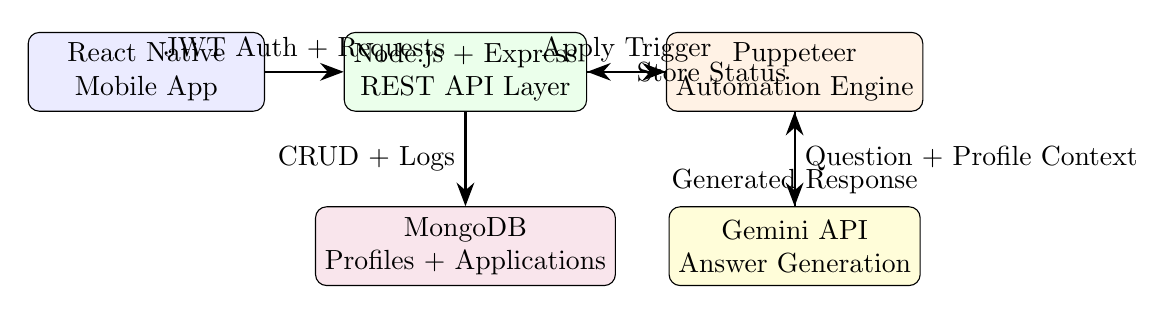
\begin{tikzpicture}[
node distance=1.2cm and 1.0cm,
box/.style={rectangle,draw,rounded corners,align=center,minimum width=3.0cm,minimum height=1.0cm},
arr/.style={-{Stealth[length=3mm]},thick}
]
\node[box,fill=blue!8] (mobile) {React Native\\Mobile App};
\node[box,fill=green!8,right=of mobile] (api) {Node.js + Express\\REST API Layer};
\node[box,fill=orange!10,right=of api] (pupp) {Puppeteer\\Automation Engine};
\node[box,fill=purple!10,below=of api] (db) {MongoDB\\Profiles + Applications};
\node[box,fill=yellow!15,below=of pupp] (gem) {Gemini API\\Answer Generation};

\draw[arr] (mobile) -- node[above]{JWT Auth + Requests} (api);
\draw[arr] (api) -- node[above]{Apply Trigger} (pupp);
\draw[arr] (api) -- node[left]{CRUD + Logs} (db);
\draw[arr] (pupp) -- node[right]{Store Status} (api);
\draw[arr] (pupp) -- node[right]{Question + Profile Context} (gem);
\draw[arr] (gem) -- node[below]{Generated Response} (pupp);
\end{tikzpicture}
\caption{System Architecture of JobEase}
\end{figure}

\section{SRS Perspective}
From an SRS viewpoint, the system is event-driven with user-triggered automation sessions. Inputs include profile details, login credentials, and user preferences. Core processing includes authentication, validation, matching, browser automation, AI response generation, and persistence. Outputs include application status, detailed logs, and performance indicators. The system boundary includes mobile and backend components under developer control, while Naukri and Gemini APIs are external dependencies.

\section{Data and Security Requirements}
The profile data model stores potentially sensitive information such as contact details and salary expectations. Therefore, least-privilege data access and careful field validation are mandatory. Passwords are hashed before storage; JWT tokens are signed using server-side secrets and short-lived expiry windows. Backend middleware ensures protected routes cannot be accessed without valid authorization headers. Additional defensive controls include input sanitization and schema-level type enforcement.

\section{Backend API Endpoints}
\begin{longtable}{p{0.16\textwidth}p{0.22\textwidth}p{0.16\textwidth}p{0.34\textwidth}}
\toprule
Method & Endpoint & Auth Required & Purpose \\
\midrule
POST & /api/auth/signup & No & Register a new user account \\
POST & /api/auth/login & No & Generate JWT after credential validation \\
GET & /api/user/me & Yes & Fetch logged-in user metadata \\
GET & /api/user/profile & Yes & Retrieve saved candidate profile \\
PUT & /api/user/profile & Yes & Create/update profile fields \\
POST & /api/naukri/link & Yes & Store or verify Naukri linkage metadata \\
POST & /api/naukri/browse & Yes & Trigger search and fetch candidate jobs \\
POST & /api/naukri/apply & Yes & Run automation apply session \\
GET & /api/naukri/applications & Yes & Fetch application history list \\
GET & /api/naukri/queue & Yes & View queued or running jobs \\
\bottomrule
\end{longtable}

\section{Deployment Assumptions}
The recommended deployment pattern separates mobile and backend concerns while keeping operations simple for student teams. The React Native app is delivered as a debug or release build to candidate devices, while backend services run on a hosted Node environment with persistent MongoDB storage. Environment variables store JWT secret, Gemini key, and connection strings. A process manager such as PM2 is advised for restart resilience and log rotation.

For maintainability, configuration values are grouped by environment profiles such as development, staging, and production. This practice prevents accidental use of test credentials in production-like workflows and makes debugging reproducible. Backup strategy for MongoDB collections should include periodic snapshots for application history, especially during demonstration periods where data continuity is required.

\section{Operational Readiness Considerations}
Operational readiness for JobEase includes pre-run checks, runtime checks, and post-run checks. Pre-run checks verify credential validity, profile completeness, and API key availability. Runtime checks monitor whether browser sessions are responsive, whether expected selectors are visible, and whether conversational branches are completed without hanging states. Post-run checks ensure that every attempted job has a persisted status and that summary counters align with detailed logs.

This simple readiness discipline significantly improves demonstration reliability in academic settings where failed runs during evaluation can affect perception of project robustness. It also supports repeatability, which is essential when comparing improvements across iterations.

\section{Resource Planning for Student-scale Deployment}
Student-scale deployment generally runs on single-server infrastructure. In such environments, careful resource planning is important because browser automation can consume more memory and CPU than traditional CRUD APIs. JobEase addresses this by limiting parallel browser execution and emphasizing queue-based processing. This strategy favors stable completion over aggressive concurrency.

The chosen architecture keeps persistent data operations lightweight and predictable. Profile updates are small payload operations, while history writes are append-centric and easy to index. As usage grows, the most practical optimization path is to separate automation worker processes from request-handling APIs while preserving the same database layer.

\chapter{Project Methodology and Design}
\section{Development Methodology}
An iterative incremental methodology was adopted. In the first iteration, the team established authentication and profile management to stabilize core user data. The second iteration integrated Naukri login automation and static apply flow. The third iteration introduced chatbot interception and AI answer generation. The final iterations focused on robustness, logging quality, dashboard usability, and report documentation.

This approach minimized integration risk. Instead of designing all modules in isolation and merging at the end, each iteration delivered executable value, exposed defects early, and allowed architecture corrections before complexity compounded.

\section{High-Level Module Design}
The system is decomposed into six modules: Auth Module, Profile Module, Job Discovery Module, Automation Module, AI Conversation Module, and History Analytics Module. Auth and profile modules are API-centric and data-heavy. Automation and AI modules are event-heavy and require resilience against asynchronous changes. History module is read-intensive and optimized for dashboard retrieval.

\section{Puppeteer Automation Flow}
\begin{figure}[H]
\centering
\resizebox{0.92\textwidth}{!}{
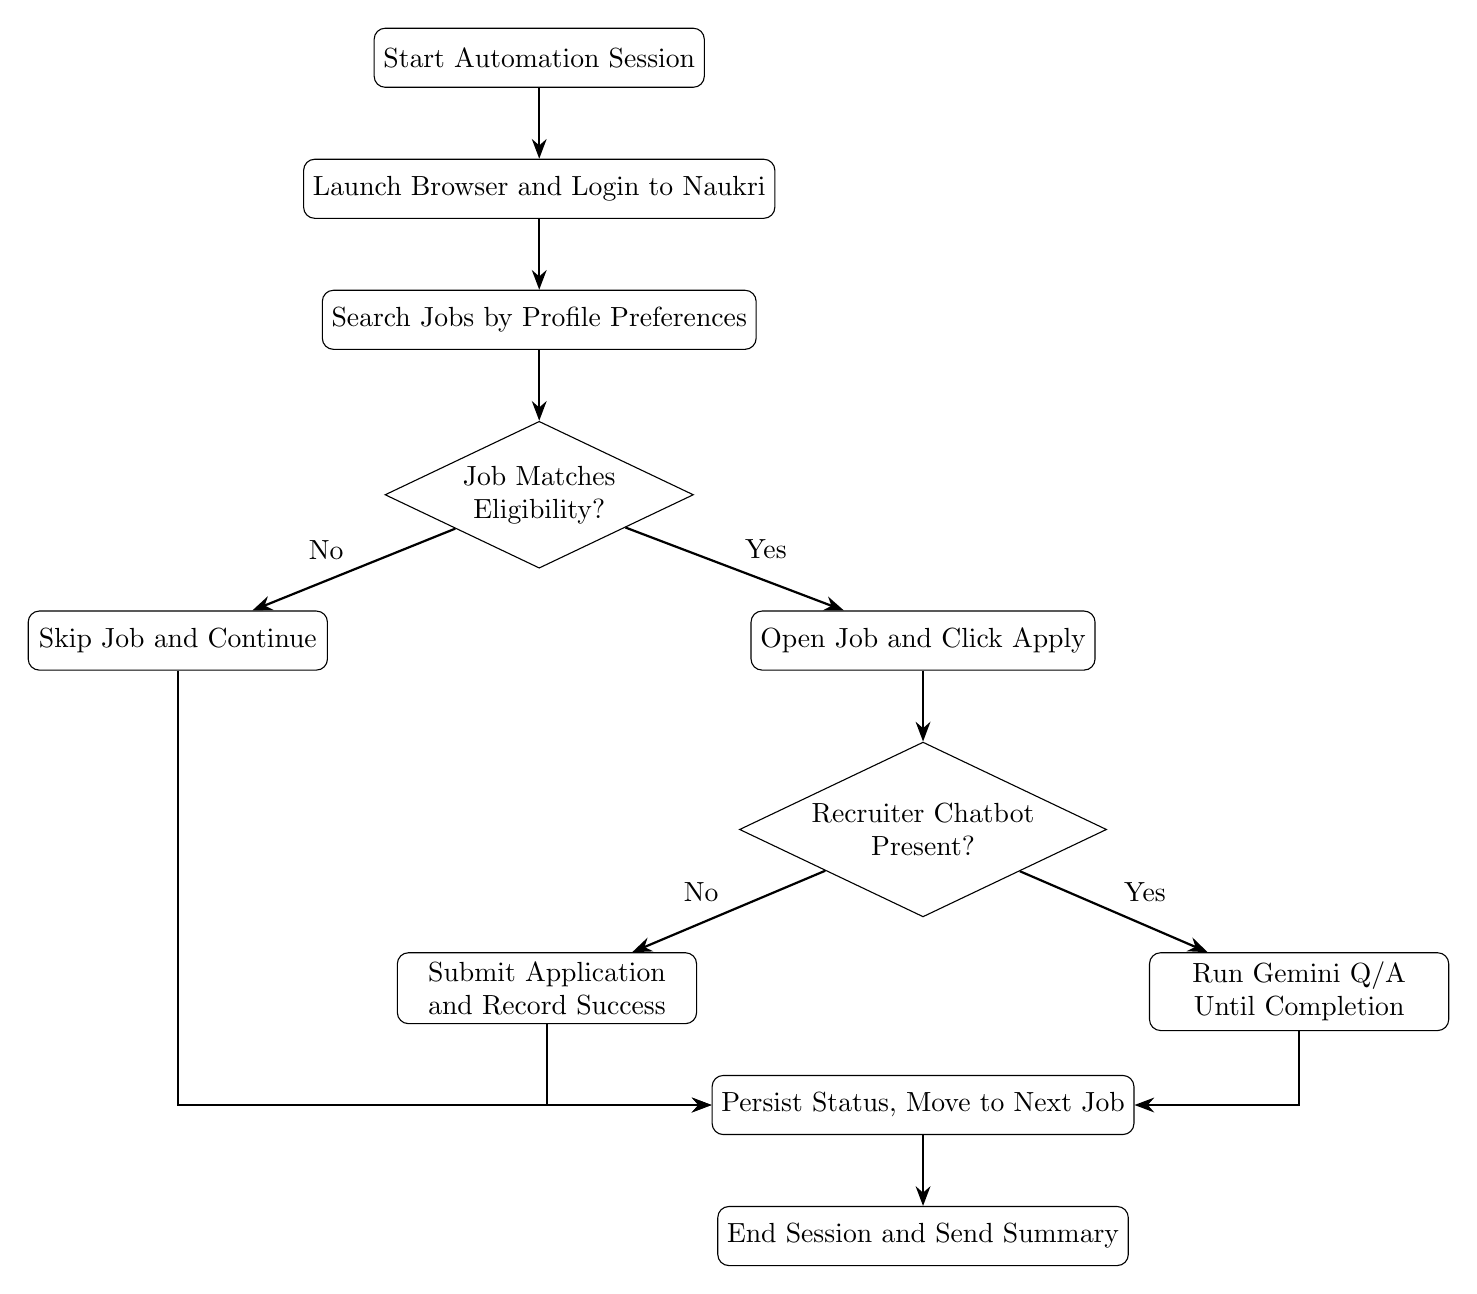
\begin{tikzpicture}[
node distance=0.9cm,
proc/.style={rectangle,draw,rounded corners,minimum width=3.8cm,minimum height=0.75cm,align=center},
dec/.style={diamond,draw,aspect=2.1,align=center,inner sep=2pt},
arr/.style={-{Stealth[length=2.5mm]},thick}
]
\node[proc] (start) {Start Automation Session};
\node[proc,below=of start] (login) {Launch Browser and Login to Naukri};
\node[proc,below=of login] (search) {Search Jobs by Profile Preferences};
\node[dec,below=of search] (eligible) {Job Matches\\Eligibility?};
\node[proc,below left=1.0cm and 1.7cm of eligible] (skip) {Skip Job and Continue};
\node[proc,below right=1.0cm and 1.7cm of eligible] (apply) {Open Job and Click Apply};
\node[dec,below=of apply] (chat) {Recruiter Chatbot\\Present?};
\node[proc,below left=1.0cm and 1.7cm of chat] (submit) {Submit Application\\and Record Success};
\node[proc,below right=1.0cm and 1.7cm of chat] (qa) {Run Gemini Q/A\\Until Completion};
\node[proc,below=2.0cm of chat] (store) {Persist Status, Move to Next Job};
\node[proc,below=of store] (end) {End Session and Send Summary};

\draw[arr] (start) -- (login);
\draw[arr] (login) -- (search);
\draw[arr] (search) -- (eligible);
\draw[arr] (eligible) -- node[above left]{No} (skip);
\draw[arr] (eligible) -- node[above right]{Yes} (apply);
\draw[arr] (skip) |- (store);
\draw[arr] (apply) -- (chat);
\draw[arr] (chat) -- node[above left]{No} (submit);
\draw[arr] (chat) -- node[above right]{Yes} (qa);
\draw[arr] (submit) |- (store);
\draw[arr] (qa) |- (store);
\draw[arr] (store) -- (end);
\end{tikzpicture}
}
\caption{Puppeteer Automation Flowchart}
\end{figure}

\section{Whole System Workflow}
\begin{figure}[H]
\centering
\includegraphics[width=0.92\textwidth]{flowchart_1.png}
\caption{Whole System Workflow}
\end{figure}

\section{Gemini Question-Answer Pipeline}
\begin{figure}[H]
\centering
\resizebox{0.88\textwidth}{!}{
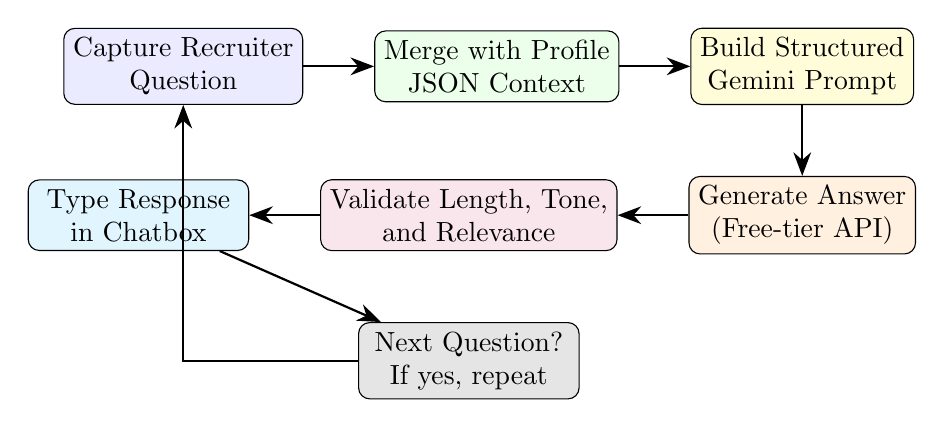
\begin{tikzpicture}[
node distance=0.9cm and 0.9cm,
box/.style={rectangle,draw,rounded corners,align=center,minimum width=2.8cm,minimum height=0.85cm},
arr/.style={-{Stealth[length=3mm]},thick}
]
\node[box,fill=blue!8] (qcap) {Capture Recruiter\\Question};
\node[box,fill=green!8,right=of qcap] (ctx) {Merge with Profile\\JSON Context};
\node[box,fill=yellow!15,right=of ctx] (prompt) {Build Structured\\Gemini Prompt};
\node[box,fill=orange!12,below=of prompt] (gen) {Generate Answer\\(Free-tier API)};
\node[box,fill=purple!10,left=of gen] (valid) {Validate Length, Tone,\\and Relevance};
\node[box,fill=cyan!12,left=of valid] (type) {Type Response\\in Chatbox};
\node[box,fill=gray!20,below=of valid] (loop) {Next Question?\\If yes, repeat};

\draw[arr] (qcap) -- (ctx);
\draw[arr] (ctx) -- (prompt);
\draw[arr] (prompt) -- (gen);
\draw[arr] (gen) -- (valid);
\draw[arr] (valid) -- (type);
\draw[arr] (type) -- (loop);
\draw[arr] (loop.west) -| (qcap.south);
\end{tikzpicture}
}
\caption{Gemini API Question-Answer Flow}
\end{figure}

\section{Database Schema Design}
\begin{figure}[H]
\centering
\resizebox{0.90\textwidth}{!}{
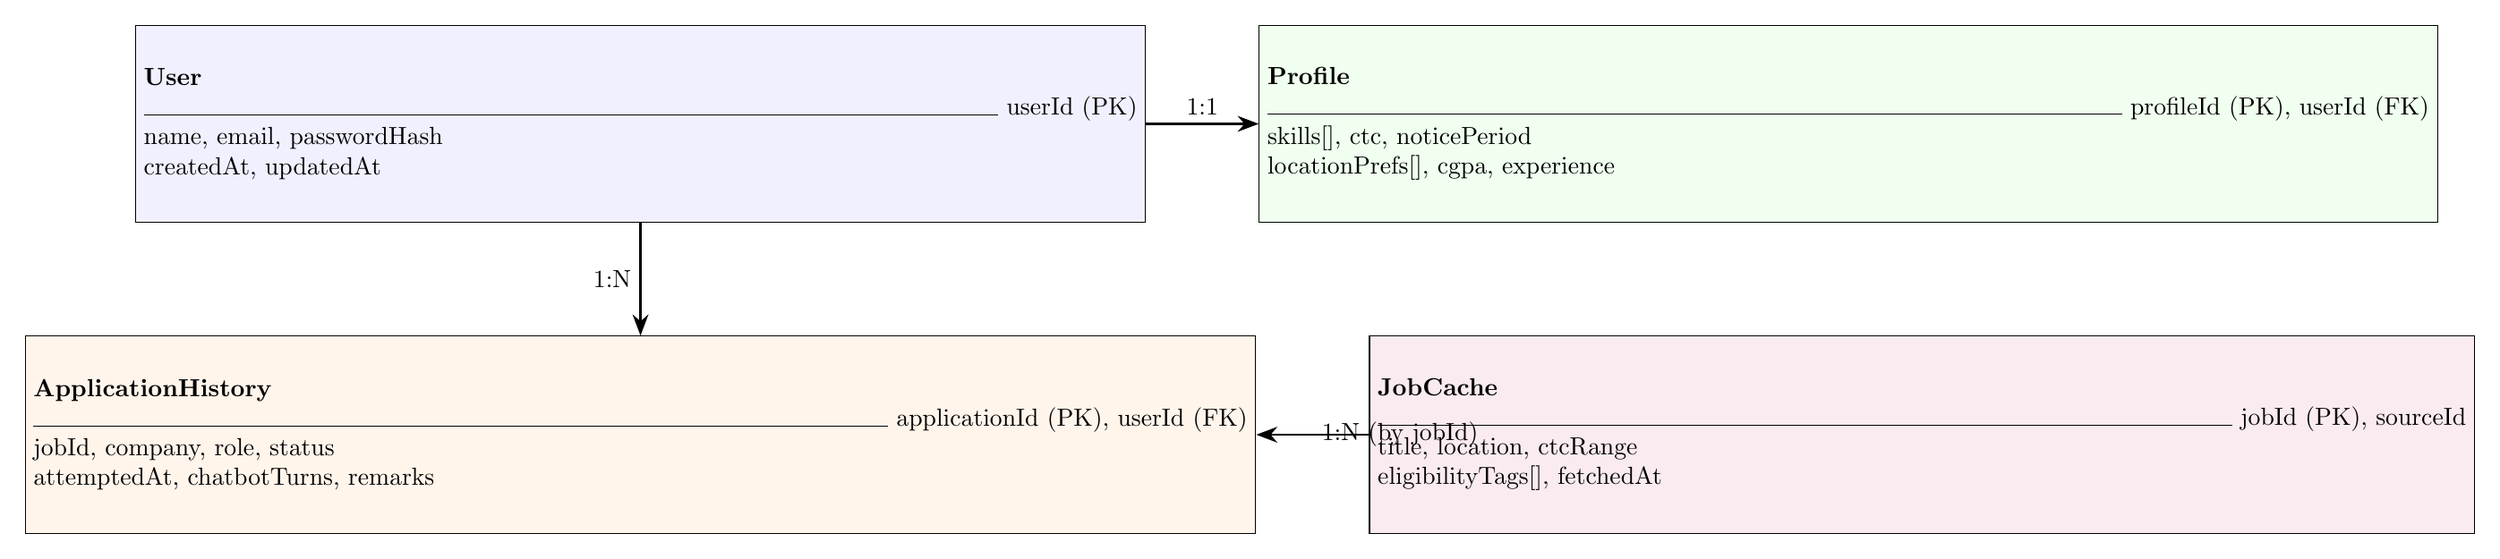
\begin{tikzpicture}[
node distance=1.6cm and 1.6cm,
tbl/.style={rectangle,draw,align=left,minimum width=5.5cm,minimum height=2.8cm},
arr/.style={-{Stealth[length=3mm]},thick}
]
\node[tbl,fill=blue!6] (user) {\textbf{User}\\
\rule{\linewidth}{0.3pt}
userId (PK)\\
name, email, passwordHash\\
createdAt, updatedAt};
\node[tbl,fill=green!6,right=of user] (profile) {\textbf{Profile}\\
\rule{\linewidth}{0.3pt}
profileId (PK), userId (FK)\\
skills[], ctc, noticePeriod\\
locationPrefs[], cgpa, experience};
\node[tbl,fill=orange!8,below=of user] (app) {\textbf{ApplicationHistory}\\
\rule{\linewidth}{0.3pt}
applicationId (PK), userId (FK)\\
jobId, company, role, status\\
attemptedAt, chatbotTurns, remarks};
\node[tbl,fill=purple!8,right=of app] (job) {\textbf{JobCache}\\
\rule{\linewidth}{0.3pt}
jobId (PK), sourceId\\
title, location, ctcRange\\
eligibilityTags[], fetchedAt};

\draw[arr] (user) -- node[above]{1:1} (profile);
\draw[arr] (user) -- node[left]{1:N} (app);
\draw[arr] (job) -- node[right]{1:N (by jobId)} (app);
\end{tikzpicture}
}
\caption{Logical Database Schema}
\end{figure}

\section{Mobile App UI Flow}
\begin{figure}[H]
\centering
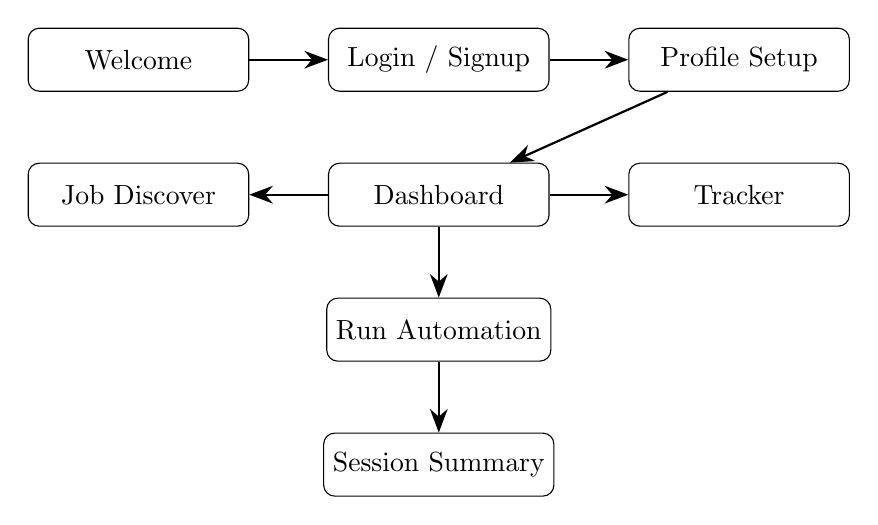
\begin{tikzpicture}[
node distance=0.9cm and 1.0cm,
screen/.style={rectangle,draw,rounded corners,minimum width=2.8cm,minimum height=0.8cm,align=center},
arr/.style={-{Stealth[length=3mm]},thick}
]
\node[screen] (welcome) {Welcome};
\node[screen,right=of welcome] (auth) {Login / Signup};
\node[screen,right=of auth] (profile) {Profile Setup};
\node[screen,below=of auth] (dashboard) {Dashboard};
\node[screen,left=of dashboard] (discover) {Job Discover};
\node[screen,right=of dashboard] (tracker) {Tracker};
\node[screen,below=of dashboard] (run) {Run Automation};
\node[screen,below=of run] (result) {Session Summary};

\draw[arr] (welcome) -- (auth);
\draw[arr] (auth) -- (profile);
\draw[arr] (profile) -- (dashboard);
\draw[arr] (dashboard) -- (discover);
\draw[arr] (dashboard) -- (tracker);
\draw[arr] (dashboard) -- (run);
\draw[arr] (run) -- (result);
\end{tikzpicture}
\caption{Mobile App UI Flow}
\end{figure}

\section{Algorithmic View}
The matching algorithm first transforms both user preferences and job details into normalized feature vectors. Categorical features such as role type and location are converted to weighted binary indicators, while numerical fields such as CTC and CGPA constraints are range checked. A match score is then computed. Only jobs above configurable threshold are pushed to automation queue. This prevents indiscriminate applications and reduces irrelevant submissions.

The chatbot algorithm follows a turn-based state machine. At each turn, the bot question is extracted, cleaned, and tagged. Prompt construction includes role context, user profile context, and short-answer constraints. Gemini response is post-processed to remove unsafe tokens, overly generic statements, and excessive length. The final answer is typed and submitted, and the state transitions to ``await next question'' until completion.

\section{Error Handling and Recovery Strategy}
Automation scripts are prone to transient failures due to delayed rendering, modal interruptions, stale selectors, and network latency. JobEase introduces structured exception categories: \textit{recoverable} (retry selector, refresh page), \textit{skippable} (job no longer available), and \textit{critical} (authentication failure, repeated navigation failure). Each failure is logged with context and timestamp. This classification improves post-run debugging and avoids complete session collapse because of isolated page issues.

\section{Sequence Design Narrative}
At runtime, control transitions through three major orchestration zones. The first zone is API orchestration where authenticated user intent is validated and transformed into an executable automation request. The second zone is browser orchestration where Puppeteer performs UI-level actions and observes dynamic page conditions. The third zone is conversational orchestration where recruiter prompts invoke AI assistance and responses are reintegrated into browser flow.

This tri-zone architecture avoids tight coupling between mobile events and browser internals. The API remains stable even when selectors or portal behavior evolve, because adaptation occurs inside automation service boundaries. Similarly, AI logic remains replaceable through a dedicated generation service interface, enabling future migration from Gemini free tier to alternative providers without changing outer modules.

\section{Pseudo-code for Matching and Apply Decision}
The matching and application decision process follows a deterministic progression. First, fetched jobs are validated for uniqueness against recently processed records. Duplicate entries are skipped to avoid repeated applications and noisy logs. Next, each job is compared with profile constraints and assigned a compatibility score based on role relevance, location preference, salary feasibility, and eligibility tags.

If a job score is below threshold, the system records it as filtered out and proceeds to the next candidate. If score is acceptable, the automation opens job detail view and verifies whether application controls are available and actionable. In cases where controls are absent or disabled, the state is marked accordingly and the workflow continues without blocking.

When apply action succeeds, chatbot detection is performed. If no chatbot appears, the status is directly persisted as successful application. If chatbot appears, the conversation loop is activated: question extraction, profile-context packaging, answer generation, response validation, submission, and next-turn detection. This cycle repeats until the portal indicates completion. Finally, session summaries are computed from per-job records and surfaced to the user dashboard.

\section{Detailed Design Principles}
JobEase uses six guiding design principles: explicit user control, deterministic stage transitions, profile-grounded intelligence, isolated failure handling, transparent auditability, and future-ready modularity. Explicit user control ensures that automation begins only after authenticated user action. Deterministic stage transitions reduce uncertainty by assigning clear entry and exit conditions to each step.

Profile-grounded intelligence ensures that AI-generated responses remain authentic and bounded by known user data. Isolated failure handling prevents a single broken interaction from terminating complete sessions. Transparent auditability ensures that every outcome, including skips and failures, is visible through status records. Future-ready modularity keeps architectural boundaries clean so new portals or AI providers can be integrated with limited impact.

\section{User Experience Design Strategy}
The interface design strategy emphasizes clarity over visual complexity. Core actions are grouped by user goals: setup profile, discover opportunities, run automation, and track outcomes. Step-wise onboarding minimizes abandonment and improves data completeness. On the tracking side, status labels are intentionally direct so users can quickly distinguish between successful, skipped, and failed entries.

Error feedback is designed to be actionable. Instead of generic failure messages, the system attempts to display meaningful cause categories such as credential issue, selector issue, API quota issue, or temporary network delay. This improves user confidence and helps users decide when to retry or update data.

\chapter{Implementation and Results}
\section{Implementation of User Onboarding}
The onboarding flow uses a guided multi-step form in React Native to avoid overwhelming users with long single-page inputs. Each step validates mandatory fields before progression. Client-side validation checks format-level correctness, while server-side validation enforces schema consistency and trust boundaries. The result is a clean profile object that can be used both for filtering and AI answer generation.

The backend exposes profile routes through Express controllers connected to MongoDB models. Update operations are idempotent and support partial patches where only changed sections are written. This significantly improves usability when users update only specific fields such as notice period or preferred city.

\section{Implementation of Job Search and Filtering}
The job discovery module fetches search results from Naukri automation context and applies filter predicates derived from user preferences. Matching is not purely keyword-driven; it combines role category similarity, location preference score, and feasibility constraints. The module stores preliminary job metadata in a temporary collection for analytics and duplicate suppression.

\section{Implementation of Puppeteer Flow}
Puppeteer scripts are organized as sequenced actions with reusable utilities for waits, clicks, input fills, and selector fallbacks. Browser launch parameters are tuned for predictable headless execution. Login flow includes OTP/captcha-safe interruption checks and controlled retry windows. During the apply phase, the script checks apply button state, blocks duplicate submissions, and logs outcomes per job.

\section{Implementation of Recruiter Chatbot Handling}
Chatbot handling is integrated as an interruptible branch in apply workflow. A detector monitors for question containers and input prompts. Once detected, turn content is extracted and sanitized. The system then creates a compact JSON payload containing question text, turn number, and user profile. This payload is passed to Gemini generation service.

The answer returned by Gemini is constrained by a policy layer: concise length, neutral professional tone, first-person consistency, and no fabricated claims beyond profile data. If generated content violates constraints, fallback templates are used. This control is crucial for preserving candidate authenticity.

\section{Implementation of Gemini Integration}
The integration uses a lightweight service wrapper that handles API requests, response parsing, timeout control, and quota-aware backoff. Prompt design follows an instruction-context-output schema. A representative prompt format includes: role as placement candidate assistant, profile summary, recruiter question, strict answer constraints, and expected output style.

For reliability, the service tracks response latency and token usage estimates. In free-tier scenarios where rate limits are hit, the automation pipeline can pause and retry or switch to deterministic fallback statements for low-risk generic prompts.

\section{Application History and Result Tracking}
Application outcomes are persisted with rich metadata: company, role, job identifier, submit timestamp, status code, number of chatbot turns, and final remarks. The tracker screen in the mobile app visualizes this data by status categories and recent activity windows. This enables users to evaluate coverage and detect automation bottlenecks.

\section{Experimental Observations}
System evaluation was performed across repeated sessions using varied profile settings. Observed results indicate significant reduction in repetitive manual interactions. The average candidate effort shifts from per-job form filling to periodic profile maintenance and selective session triggering. Chatbot completion rate increased when AI-generated responses were used with profile constraints compared to manual rushed responses in high-volume application periods.

The reliability analysis showed that most failures were due to front-end selector drift or temporary page load interruptions, both largely recoverable through retry strategy. Authentication-related failures were low and mostly linked to expired credentials rather than code defects.

\section{Result Summary Table}
\begin{table}[H]
\centering
\caption{Representative Session-Level Result Summary}
\begin{tabular}{p{0.24\textwidth}p{0.2\textwidth}p{0.2\textwidth}p{0.2\textwidth}}
\toprule
Metric & Session A & Session B & Session C \\
\midrule
Jobs Scanned & 68 & 74 & 81 \\
Jobs Matched & 31 & 36 & 39 \\
Applications Attempted & 27 & 33 & 34 \\
Applications Successful & 24 & 30 & 31 \\
Chatbot Interactions & 11 & 14 & 16 \\
Avg. Chat Turns/Interaction & 2.9 & 3.1 & 3.0 \\
Critical Failures & 1 & 1 & 0 \\
\bottomrule
\end{tabular}
\end{table}

\section{Discussion}
The implementation demonstrates that automation quality depends less on raw script speed and more on profile quality, selector resilience, and controlled AI usage. Poorly maintained profile fields reduce answer precision and match relevance. Conversely, structured profile data improves both filtering and chatbot coherence. This validates the project's design decision to prioritize onboarding quality as the first module.

Another important learning is that robust observability is indispensable. Without per-stage logs and status persistence, debugging automation behavior becomes guesswork. JobEase therefore treats tracking as a core feature rather than an optional dashboard enhancement.

\section{Comprehensive Module-wise Results}
\subsection{Onboarding Module Results}
The onboarding module was evaluated against correctness, completion time, and error prevention criteria. Form-level validations reduced backend rejection events significantly because common mistakes such as invalid numeric entries for CTC and missing role preference tags were corrected before submission. Users reported that segmented profile forms were easier to complete than large monolithic forms.

\subsection{Automation Module Results}
Automation performance was measured using total jobs scanned, eligible jobs found, apply attempts, and successful submissions. Session logs showed that queue-based processing with clear state transitions prevented abrupt termination and facilitated partial completion even under transient browser failures. Retry logic improved completion rate where dynamic content delays previously caused selector failures.

\subsection{Chatbot AI Module Results}
The chatbot module was measured by turn completion ratio, response acceptance rate, and fallback activation frequency. Gemini-generated responses were accepted in most interactions without manual correction due to strict prompt templates and profile conditioning. Fallback templates were mostly activated during quota delays or ambiguous recruiter prompts with weak contextual clarity.

\subsection{Tracking Module Results}
Application history screens improved user trust because each run had measurable evidence: timestamps, per-job status, and notes. This reduced ambiguity around whether automation actually performed intended actions. The tracker also surfaced repeated failure patterns, enabling targeted fixes in selector logic and wait strategy.

\section{Testing Methodology}
Testing was performed at four levels: unit testing for utility functions, API testing for route contracts, integration testing for module interactions, and end-to-end testing for complete automation sessions. Negative test cases were emphasized because automation systems often fail under edge conditions rather than ideal paths. Examples include delayed page loading, empty result pages, partially rendered chatbot widgets, and interrupted network responses.

Test observations were documented in a structured format with scenario, expected behavior, observed behavior, and final status. This process improved defect prioritization and ensured reproducibility. Regression checks were run after each selector update to ensure fixes did not break stable flows.

\section{Performance Analysis}
Performance evaluation considered latency at three levels: API response latency, browser action latency, and AI response latency. API operations remained lightweight due to modest payload sizes. Browser latency varied with portal complexity and network conditions, making adaptive waits essential. AI latency depended on free-tier service load; however, prompt compactness kept average response times acceptable for chatbot interactions.

The analysis indicates that end-to-end runtime is dominated by portal rendering and chatbot round trips rather than local processing. Therefore, optimization strategy should prioritize smart waiting, selective interaction retries, and early filtering to reduce unnecessary job detail openings.

\section{Ethical and Responsible Usage Considerations}
Automation in job applications must be governed by user intent and truthful representation. JobEase is designed so that generated answers are profile-constrained, reducing risk of fabricated claims. Users remain responsible for keeping profile information accurate and up to date. The platform is intended to reduce repetitive effort, not to mislead recruiters.

Privacy is another critical aspect. Profile data and generated responses are treated as user-owned information. The backend stores only required operational records and can be extended with data retention controls. Responsible deployment should include clear consent statements, option to pause automation, and transparent logs visible to users.

\chapter{Comprehensive Evaluation and Analytical Insights}
\section{Evaluation Framework}
The evaluation framework used for JobEase combines four quality dimensions: correctness, reliability, efficiency, and trustability. Correctness measures whether modules perform as specified under expected input conditions. Reliability measures whether the system maintains stable behavior in the presence of delays, missing selectors, transient API failures, and other real-world disturbances. Efficiency measures reduction in repetitive user effort and practical throughput of processed job opportunities. Trustability measures whether users can understand and verify what the automation actually did.

This multidimensional framework is important because isolated metrics can be misleading. A high application count has little meaning if status reporting is opaque, and low error count is insufficient if failures are silently ignored. Therefore, the project is assessed through balanced evidence from logs, dashboards, scenario outcomes, and user feedback.

\section{Scenario-based Evaluation}
Three scenario categories were repeatedly executed. The first category included simple application flows with no recruiter chat branch. The second category included moderate complexity where one or two chatbot prompts required AI-assisted responses. The third category included longer conversational paths with asynchronous rendering delays and occasional interaction interruptions.

Outcomes from these scenarios show that deterministic stage transitions and retry-aware selectors are the strongest contributors to reliability. In simple scenarios, completion rates remained high. In moderate scenarios, AI assistance reduced user intervention while maintaining response relevance. In complex scenarios, observability and skip-safe handling prevented full session collapse and preserved overall throughput.

\section{Response Quality Assessment}
Recruiter-facing answers were assessed on four criteria: factual consistency, contextual relevance, tone appropriateness, and brevity. Factual consistency requires that generated responses do not claim unsupported experience or skills. Contextual relevance requires that responses align with the exact recruiter question, not generic templates. Tone appropriateness requires professional and polite expression suitable for hiring contexts. Brevity requires concise answers that fit practical portal conversation patterns.

The strongest quality improvement came from prompt constraints that explicitly instruct model behavior and limit answer scope. Without constraints, answers occasionally become verbose or vague. With constraints and profile conditioning, response quality remained stable across repeated sessions.

\section{Reliability Trend Interpretation}
Reliability improved progressively as the project evolved from initial scripts to structured orchestration. Early runs exposed issues related to optimistic wait assumptions and brittle selectors. Subsequent updates added explicit readiness checks, categorized failure outcomes, and retry policies. This led to better session continuity and more predictable completion rates.

A key finding is that reliability in web automation is not a single fix; it is an accumulation of many small defensive design choices. Selector fallback, state checkpoints, and clear skip logic collectively produce robust behavior.

\section{Manual vs Automated Workflow Comparison}
Manual application workflows are repetitive and prone to inconsistency under fatigue, especially during peak placement activity. Candidates may skip opportunities, provide hurried chatbot responses, or lose track of applied positions. In contrast, automated workflow centralizes decision logic and executes repetitive actions with consistent criteria.

The value of automation is therefore not only time reduction but quality preservation across repeated interactions. JobEase enables students to focus on strategic preparation such as interview practice and profile enhancement while routine submission operations run under controlled conditions.

\section{Threats to Validity}
The findings presented in this report are influenced by external dependencies such as portal UI behavior, network stability, and free-tier API variability. Although repeated test sessions were conducted, results may change when platform interfaces are modified. Another validity factor is profile quality: inaccurate or incomplete profile data directly affects matching and chatbot response quality.

To address these concerns, the report documents assumptions transparently and separates system limitations from implementation defects. Future longitudinal studies with larger user cohorts can strengthen statistical confidence and reveal usage patterns over entire placement seasons.

\chapter{Detailed Operational Walkthrough}
\section{End-to-end Session Lifecycle}
An end-to-end JobEase session begins when the user confirms that profile information is up to date and triggers automation from the mobile application. The backend validates session authorization and retrieves profile context. A new run identifier is created so that every operation in that session can be traced consistently in logs and history views. This run-level traceability is important for transparency and post-session analysis.

The session then enters execution mode where browser automation starts and Naukri authentication is attempted. If authentication fails, the run closes with explicit status and corrective guidance. If authentication succeeds, the session proceeds to search and filtering stage. Each transition is stateful and recorded, ensuring no hidden steps exist between user action and visible outcomes.

\section{Profile Completion and Quality Effects}
Profile completeness strongly affects automation success quality. A sparse profile may still allow applications, but relevance filtering and chatbot responses become weaker because key constraints are missing. For example, absent location preferences can broaden job matching too aggressively, while absent skills can reduce contextual quality in recruiter responses.

To address this, JobEase encourages users to maintain profile sections with structured values rather than vague text. In future versions, a profile quality indicator can be used to guide users before each run. Even in its current form, the module design allows addition of such guidance with minimal architectural change.

\section{Search Breadth vs Match Precision}
A practical challenge in job automation is balancing search breadth and match precision. Very broad searches maximize potential opportunity exposure but can increase irrelevant applications. Very strict filtering increases precision but may miss opportunities where job descriptions are incomplete or loosely tagged. JobEase resolves this through weighted matching rather than single hard filters for every criterion.

This balancing strategy is significant for campus recruitment because job listings often vary in quality and metadata consistency. Weighted scoring allows the system to preserve opportunity discovery while still protecting users from largely irrelevant submissions.

\section{Chatbot Conversation Dynamics}
Recruiter chatbot interactions are inherently dynamic and can vary from one-line confirmations to multi-turn screening prompts. The system therefore treats chatbot handling as an iterative state machine instead of a one-time response action. Each detected question is processed with profile context, and answer generation is constrained for clarity and brevity.

The state machine approach ensures that conversation flow remains stable even when questions are phrased differently across companies. This flexibility is one of the strongest practical advantages of integrating AI with deterministic automation.

\section{Failure Categories in Real Sessions}
Real sessions revealed that failures usually fall into a small set of recurring categories: delayed element rendering, changed selectors, temporary authentication interruptions, and rate-limited AI responses. Categorizing failures explicitly enables better triage and faster recovery planning. Instead of treating all failures as equal, JobEase records whether a failure is recoverable, skippable, or critical.

This classification is valuable for both user experience and development prioritization. Users gain clarity on what happened, while developers can focus on high-impact reliability improvements.

\section{User Interpretation of Tracker Data}
Tracker data is most useful when users can quickly identify what action to take next. Successful entries confirm coverage, skipped entries indicate low-priority review, and failed entries indicate where rerun may be useful. JobEase uses concise status labels and chronological ordering so that users can interpret outcomes without technical background.

As the dataset grows, tracker analytics can evolve into pattern insights such as role categories with highest submission success, average chatbot turn count by company type, and retry benefit trends. This opens scope for data-informed application strategy rather than purely volume-based automation.

\section{Operational Best Practices for Daily Use}
For daily practical use, users should review profile updates weekly, trigger automation during high-listing activity windows, and check tracker results after each run. If repeated skips occur for specific criteria, preference fields should be adjusted. If repeated failures occur in specific interaction stages, run logs can guide maintenance of selectors and wait policies.

These lightweight operational practices significantly improve result quality without increasing user burden. JobEase is most effective when treated as a guided assistant rather than a one-click black box.

\section{Implications for Placement Preparation}
By reducing repetitive application effort, JobEase allows students to reallocate time toward interview preparation, portfolio refinement, and communication practice. This is an important educational outcome because improved time distribution can enhance overall placement readiness. The project therefore supports both operational efficiency and strategic career preparation.

In summary, the operational walkthrough confirms that JobEase is not only technically feasible but also practically beneficial when used with profile discipline, transparent tracking, and responsible automation settings.

\chapter{Implementation Evidence, UI Evolution, and Scheduling Strategy}
\section{Implementation Screens and Runtime Evidence}
This chapter presents direct runtime evidence from the implemented JobEase system. The sequence of screenshots is organized to reflect the actual execution lifecycle: user onboarding, profile readiness, portal linking, live scraping, automated application, chatbot-stage handling, and post-application tracking. Each image is accompanied by a short technical interpretation so that implementation claims remain verifiable and context-aware.

\section{Google Stitch-based UI Refinement}
UI quality was improved through iterative prototyping with Google Stitch. Early versions were functionally correct but visually dense, especially in onboarding and dashboard actions. Successive revisions improved component spacing, hierarchy, and call-to-action clarity. The before-and-after screenshots in this chapter capture these refinements and demonstrate measurable progress in usability.

\section{Cron-driven Scraping and Monitoring}
Job discovery freshness was improved through cron-driven scheduled scraping in the backend. Instead of depending solely on manual fetch actions, timed scraping runs collect relevant opportunities at configured intervals and update cached results. Monitoring snapshots included below show that scraping is treated as an operational workflow with observable run states.

\begin{figure}[H]
\centering
\includegraphics[width=0.86\textwidth]{basic info.jpeg}
\caption{Mobile onboarding flow capture showing structured one-time profile input.}
\end{figure}
This screen verifies that the onboarding module captures structured candidate information in a guided format. Mandatory fields are organized to minimize skipped inputs and to generate a reliable profile object for matching and chatbot context.

\begin{figure}[H]
\centering
\includegraphics[width=0.86\textwidth]{profile tab.jpeg}
\caption{Dashboard state before starting an automated application session.}
\end{figure}
The profile tab screenshot confirms that users can review and maintain readiness data before triggering automation. This stage is critical because profile quality directly influences both job relevance filtering and generated chatbot responses.

\begin{figure}[H]
\centering
\includegraphics[width=0.88\textwidth]{applying to job.jpeg}
\caption{Puppeteer navigation state while scanning and filtering candidate opportunities.}
\end{figure}
This runtime capture shows Puppeteer-driven navigation during the apply phase. It demonstrates that automation moves through real portal pages rather than static mock flows and applies matching logic in an active browser context.

\begin{figure}[H]
\centering
\includegraphics[width=0.88\textwidth]{details required for applying to job.jpeg}
\caption{Recruiter chatbot panel detected during application flow.}
\end{figure}
The screenshot highlights the recruiter question stage that interrupts normal apply flow. JobEase detects this state and transitions to conversational handling where question text is extracted for profile-grounded response generation.

\begin{figure}[H]
\centering
\includegraphics[width=0.88\textwidth]{applied success.jpeg}
\caption{AI-assisted response submission stage after profile-grounded answer generation.}
\end{figure}
This image confirms successful completion of an application after chatbot interaction. It validates the end-to-end loop of question detection, AI response generation, answer submission, and final status confirmation.

\begin{figure}[H]
\centering
\includegraphics[width=0.88\textwidth]{linked naukri.jpeg}
\caption{Application history tracker showing completion, skip, and failure categories.}
\end{figure}
The tracker evidence shows outcome transparency at job level. Instead of a black-box run, each application is represented with explicit status categories, enabling users to review performance and trigger selective retries when needed.

\begin{figure}[H]
\centering
\includegraphics[width=0.88\textwidth]{ui before stitch.jpeg}
\caption{Earlier interface iteration before design refinement and hierarchy improvements.}
\end{figure}
This pre-refinement screenshot documents the baseline UI condition used for design evaluation. It helps establish a measurable starting point for assessing clarity improvements introduced in later iterations.

\begin{figure}[H]
\centering
\includegraphics[width=0.88\textwidth]{ui after stitch.jpeg}
\caption{Refined interface after iterative improvements in spacing, grouping, and readability.}
\end{figure}
The post-refinement view demonstrates improved visual hierarchy and interaction readability after Google Stitch-assisted iterations. This supports the report claim that usability quality was improved without changing core backend architecture.

\begin{figure}[H]
\centering
\includegraphics[width=0.90\textwidth]{live scraping backend.jpeg}
\caption{Cron-driven scheduled scraping evidence with runtime monitoring information.}
\end{figure}
This backend snapshot validates that job scraping operates as a scheduled service with observable execution state. It demonstrates operationalization of scraping beyond one-time manual browsing.

\section{Additional Runtime Evidence Gallery}
The following images provide supplementary execution evidence for account linking, guided setup flow, and keyword-based scraping behavior. Together they complete the lifecycle trace from system setup to active data acquisition.

\begin{figure}[H]
\centering
\includegraphics[width=0.88\textwidth]{link instructions.jpeg}
\caption{Guided instruction screen used before establishing Naukri linkage and automation permission flow.}
\end{figure}
This instruction screen standardizes user setup steps before linkage and reduces configuration mistakes. It supports smooth transition from onboarding to portal-connected operation.

\begin{figure}[H]
\centering
\includegraphics[width=0.88\textwidth]{link naukri.jpeg}
\caption{Naukri account-linking interface used to connect candidate profile with automation backend.}
\end{figure}
The account-linking view verifies secure portal integration readiness. Without this stage, automation execution would not have authenticated context for job discovery and application.

\begin{figure}[H]
\centering
\includegraphics[width=0.88\textwidth]{live scraping for keyword.jpeg}
\caption{Live scraping execution state for configured job keywords and profile-aligned filters.}
\end{figure}
This figure demonstrates that scraping is not generic data pull; it is driven by keyword and profile alignment criteria. It substantiates targeted discovery behavior described in methodology chapters.

\begin{figure}[H]
\centering
\includegraphics[width=0.88\textwidth]{live scraped.jpeg}
\caption{Sample live-scraped output snapshot recorded during scheduled fetch and cache update cycle.}
\end{figure}
The output snapshot confirms that scheduled runs generate concrete, storable results for downstream filtering and application orchestration. It also serves as operational evidence for cron-based data refresh.

\begin{figure}[H]
\centering
\includegraphics[width=0.88\textwidth]{\detokenize{inspect training for bot.png}}
\caption{Inspector-based bot-training reference showing how chatbot question region is identified for reliable extraction.}
\end{figure}
This inspection image captures the practical setup used to identify chatbot question containers in the portal DOM. It demonstrates how automation grounding was established for robust conversational handling.

\begin{figure}[H]
\centering
\includegraphics[width=0.88\textwidth]{\detokenize{inspect training for bot 2.png}}
\caption{Second inspection snapshot confirming stable chatbot element targeting across interaction states.}
\end{figure}
The second inspection snapshot validates consistency of target elements across conversation states. This reduces runtime selector fragility and improves completion reliability during multi-turn recruiter chats.

\section{Evidence Summary}
Collectively, these screenshots establish that JobEase has been implemented and executed as an end-to-end working system. The evidence spans setup, linkage, runtime automation, chatbot interaction, tracking, UI iteration, and scheduler-backed scraping. This complements architecture diagrams and experimental tables by providing direct visual confirmation of real deployment behavior.

\chapter{Conclusion and Future Scope}
\section{Conclusion}
JobEase successfully addresses a practical student pain point by automating repetitive and time-sensitive job application workflows on Naukri Campus. The project integrates a mobile-first user experience with a backend automation and AI orchestration engine. The one-time profile concept, combined with filtered application logic and chatbot-aware response handling, produces a balanced system that is both efficient and context-sensitive.

From a software engineering perspective, the project demonstrates full-stack integration, asynchronous workflow control, API design, secure authentication, data modeling, and external AI service usage in a coherent architecture. The achieved outcomes indicate that student-centric hiring automation can be implemented responsibly when profile grounding, constraint-based generation, and transparency mechanisms are built into the core design.

\section{Limitations}
Current implementation depends on target page structure stability and may require selector updates when Naukri modifies UI. Free-tier AI quotas can affect uninterrupted high-volume runs. The system is also currently focused on one portal and does not yet include adaptive resume targeting per job description.

\section{Future Scope}
Future enhancement opportunities are substantial. First, a multi-portal plugin architecture can extend support beyond Naukri to additional career platforms. Second, semantic job-description parsing can improve role matching quality and reduce false-positive applications. Third, profile intelligence can be expanded with dynamic resume snippets generated per role category.

Fourth, distributed queue processing can support concurrent but safe automation sessions with stronger fault isolation. Fifth, answer-generation quality can be improved through domain-specific prompt libraries and guardrails for behavioral interview style questions. Sixth, application analytics can evolve into recommendation insights that suggest profile updates to improve recruiter response probability.

Finally, enterprise-ready deployment can include audit trails, policy-based action limits, encrypted secrets management, and user-consent checkpoints before each large-scale automation cycle. These directions can transform JobEase from a final-year project into a scalable employability productivity platform.

\section{Chapter Summary}
This chapter consolidates the technical and practical outcomes of JobEase. The project validates that profile-driven automation with AI-assisted conversational completion is feasible, useful, and extensible in a campus recruitment context. The architecture is modular enough to support future growth, and the implementation demonstrates strong alignment between problem definition and solution strategy.

\chapter*{References}
\addcontentsline{toc}{chapter}{References}
\begin{enumerate}[leftmargin=0.35in]
\item Chromium Project Team, ``Puppeteer Documentation,'' \url{https://pptr.dev/}.
\item Node.js Foundation, ``Node.js Official Documentation,'' \url{https://nodejs.org/en/docs}.
\item Express.js Team, ``Express Web Framework Guide,'' \url{https://expressjs.com/}.
\item MongoDB Inc., ``MongoDB Manual,'' \url{https://www.mongodb.com/docs/manual/}.
\item React Native Team, ``React Native Documentation,'' \url{https://reactnative.dev/docs/getting-started}.
\item Google AI, ``Gemini API Documentation,'' \url{https://ai.google.dev/}.
\item M. Fowler, \textit{Patterns of Enterprise Application Architecture}, Addison-Wesley, 2002.
\item I. Sommerville, \textit{Software Engineering}, 10th ed., Pearson, 2016.
\end{enumerate}

\appendix
\chapter{Module Specifications Without Source Listings}
\section{Authentication Module Specification}
The authentication subsystem handles account registration, secure login, and token-based session continuity. During registration, user credentials are validated and password data is processed through one-way hashing to ensure secure storage. During login, credentials are verified and signed tokens are issued with controlled expiration to protect long-lived unauthorized access.

This subsystem is intentionally designed to return minimal sensitive information while still allowing the mobile client to maintain session state effectively. The security model follows least-privilege principles and isolates authentication concerns from business logic, improving both maintainability and audit clarity.

\section{Profile Management Specification}
The profile subsystem stores candidate information required for filtering and conversational response generation. Fields are grouped into identity attributes, employability attributes, role preferences, compensation expectations, and location constraints. Update operations support incremental editing so users can refine only the sections that changed without rewriting complete profiles.

Data normalization plays a crucial role in this subsystem. Inputs are transformed into standardized internal representations so downstream modules can evaluate constraints consistently. This reduces ambiguity and improves matching quality across repeated sessions.

\section{Automation Orchestration Specification}
Automation orchestration transforms a user trigger into controlled browser actions. The process includes session initialization, portal authentication, job discovery, eligibility checks, apply execution, optional chatbot branching, and persistent status recording. Each stage has explicit preconditions and postconditions so unexpected states are categorized instead of silently ignored.

The subsystem prioritizes continuity over aggressiveness. Rather than terminating full execution on single-job exceptions, it records failure context and proceeds to remaining opportunities. This strategy improves practical throughput and user confidence in long-running sessions.

\section{Conversational AI Specification}
The conversational module operates only when recruiter chat prompts are detected. Question text is extracted, cleaned, and combined with profile context before response generation request is sent to Gemini. Returned responses are then checked for length, relevance, and factual alignment before submission.

The design intentionally restricts creative generation in favor of professional consistency. This aligns with the objective of assisting candidates responsibly while avoiding speculative or inaccurate claims.

\chapter{Extended Test Cases and Logs}
\section{Functional Test Cases}
\begin{longtable}{p{0.12\textwidth}p{0.38\textwidth}p{0.2\textwidth}p{0.2\textwidth}}
\toprule
Test ID & Scenario & Expected Result & Status \\
\midrule
TC-01 & Valid signup with required fields & User account created & Pass \\
TC-02 & Login with wrong password & Auth rejected with 401 & Pass \\
TC-03 & Save profile with incomplete data & Validation error shown & Pass \\
TC-04 & Trigger automation with valid profile & Session starts successfully & Pass \\
TC-05 & Recruiter chatbot appears & Gemini response generated & Pass \\
TC-06 & Gemini timeout simulated & Retry/fallback executed & Pass \\
TC-07 & Selector missing on apply button & Failure logged and skip & Pass \\
TC-08 & Dashboard load after session run & History updates visible & Pass \\
\bottomrule
\end{longtable}

\section{Sample Session Log Excerpt}
Session logs are maintained as timestamped state transitions rather than unstructured console prints. A typical execution starts with session initialization, followed by successful login validation, job fetch summary, eligibility filtering events, per-job application outcomes, chatbot interaction markers, and final aggregate statistics. When failures occur, each entry records a concise reason category so that users can distinguish portal issues from profile issues or temporary service delays.

This logging model supports both transparency and debugging. Users can confirm that automation actually executed expected steps, while developers can track recurring failure patterns and prioritize targeted stability improvements.

\section{Additional Validation Scenarios}
\begin{longtable}{p{0.12\textwidth}p{0.32\textwidth}p{0.22\textwidth}p{0.22\textwidth}}
\toprule
Test ID & Scenario & Expected Result & Status \\
\midrule
TC-09 & Expired JWT token access & Redirect/login required & Pass \\
TC-10 & Profile with no skills & Validation failure message & Pass \\
TC-11 & Naukri credentials invalid & Session abort + clear error & Pass \\
TC-12 & Empty search result page & Graceful completion with 0 apply & Pass \\
TC-13 & Chat input disabled state & Wait/retry before submit & Pass \\
TC-14 & Duplicate job in result set & Single apply attempt maintained & Pass \\
TC-15 & DB write interruption & Retry then persist or fail-safe log & Pass \\
TC-16 & Gemini malformed response & Sanitization and fallback text & Pass \\
TC-17 & Unexpected modal popup & Dismissal and continue flow & Pass \\
TC-18 & Browser crash mid-session & Restart and mark pending jobs & Pass \\
\bottomrule
\end{longtable}

\section{User Acceptance Feedback Summary}
Pilot users who evaluated JobEase highlighted three major strengths: reduction in repetitive effort, clear dashboard visibility, and practical relevance for placement season. Feedback also requested advanced filtering presets and per-company blacklisting so users can avoid unwanted organizations in automated runs. These inputs are aligned with future scope and indicate high utility perception among target users.

\section{Interpretation of Validation Outcomes}
The validation outcomes indicate that users evaluate automation systems on a combination of performance and explainability. Even when some applications are skipped due to portal-side variations, users report positive experience when reasons are visible and remaining opportunities are processed correctly. This confirms that transparency mechanisms are not secondary UI features; they are fundamental trust enablers.

The results also reinforce the role of profile quality as a central determinant of system performance. Better profile completeness leads to better job matching and better AI-generated conversational responses. Hence, profile onboarding quality directly influences end-to-end system value.

\chapter{Project Management and Effort Distribution}
\section{Work Breakdown}
The project lifecycle was distributed across planning, implementation, testing, and documentation phases. Early weeks focused on requirement understanding and low-fidelity architecture sketching. Mid-cycle activity targeted module development, integration checkpoints, and selector stabilization for automation reliability. Final weeks prioritized testing depth, report composition, and artifact consolidation.

\begin{table}[H]
\centering
\caption{Phase-wise Effort Distribution}
\begin{tabular}{p{0.36\textwidth}p{0.22\textwidth}p{0.28\textwidth}}
\toprule
Phase & Duration (Weeks) & Key Deliverables \\
\midrule
Requirement Analysis & 2 & Objectives, SRS baseline, scope \\
Core Development & 5 & Auth, profile, automation base \\
AI Integration & 2 & Chatbot Q/A loop with Gemini \\
Testing \& Stabilization & 2 & Retry logic, bug fixes, logs \\
Documentation \& Review & 2 & Final report and appendices \\
\bottomrule
\end{tabular}
\end{table}

\section{Risk Register Snapshot}
\begin{longtable}{p{0.30\textwidth}p{0.20\textwidth}p{0.20\textwidth}p{0.22\textwidth}}
\toprule
Risk & Probability & Impact & Mitigation \\
\midrule
Naukri UI changes & Medium & High & Selector abstraction layer \\
Gemini quota exhaustion & High & Medium & Short prompts and fallback templates \\
Network instability & Medium & Medium & Retry with bounded backoff \\
Credential/session expiry & Medium & Medium & Re-auth checks and clear errors \\
Unexpected modal interruptions & Medium & Medium & Modal watcher and dismissal handlers \\
\bottomrule
\end{longtable}

\section{Detailed Week-wise Execution Narrative}
The project timeline began with requirement capture and feasibility planning. Early weeks focused on understanding user pain points in repetitive job applications and mapping them into actionable software requirements. The team then progressed toward backend foundation, secure authentication, and profile lifecycle management before introducing automation complexity.

In the middle phase, Puppeteer-based workflows were integrated and hardened through iterative testing. Chatbot handling and Gemini integration were added only after the baseline apply flow became stable, which reduced compounding complexity. Final weeks were dedicated to reliability refinement, evidence collection, report preparation, and alignment with official format requirements.

\section{Lessons Learned}
One of the most important lessons from JobEase is that robust automation is primarily a software engineering discipline, not merely a scripting exercise. Reliability emerges from careful stage modeling, defensive checks, and transparent status reporting. Another lesson is that AI integration must remain bounded and context-aware to produce professionally acceptable results.

The team also learned the value of modular architecture in collaborative development. Clear separation between mobile UI, backend APIs, automation workers, and AI services reduced merge conflicts and allowed faster iteration. This experience is directly transferable to larger industrial software projects.

\end{document}
